\documentclass[12pt,a4paper,twoside]{article}
\usepackage[utf8]{inputenc}
\usepackage[spanish]{babel}
\usepackage{amsmath}
\usepackage{lmodern}
\usepackage{textcomp}
\usepackage{amsfonts}
\usepackage{amssymb}
\usepackage{graphicx}
\usepackage[left=2cm,right=2cm,top=2cm,bottom=2cm]{geometry}
\author{Carlos Eduardo Martínez Núñez}
% used in maketitle
\title{\textbf{Trayectoria de Proyectiles}}
\begin{document}
\maketitle
El movimiento de un proyectil es un tipo de movimiento en el cual un objeto o partícula describe una trayectoria parabólica. La posición en cualquier instante durante su recorrido, se puede determinar según las siguientes ecuaciones:
\begin{eqnarray}
x=v_{0}tcos(\theta)\nonumber\\
y=v_{0}tsin(\theta)-gt^{2}
\end{eqnarray}
El tipo de trayectoria, el alcance horizontal y la altura máxima del movimiento de un proyectil en cercanías de la superficie terrestre, dependen de los parámetros iniciales del ángulo y la velocidad inicial del lanzamiento.
\section{Dependencia del ángulo}
La siguiente actividad consiste en determinar las gráficas de las trayectorias de un proyectil en función del ángulo de lanzamiento. Se requiere especificar la velocidad inicial y el número de puntos de cada gráfica. Los ángulos tomados corresponden a $15^{o}$, $30^{o}, 45^{o}, 60^{o}, 75^{o}$ y $90^{o}$. El número de puntos para cada gráfica  corresponde a 20. El tiempo de vuelo será calculado con  la siguiente ecuación:
\begin{eqnarray}
t=\frac{2v_{0}sin(\theta)}{g}
\end{eqnarray}
Si se selecciona, por ejemplo, una velocidad inicial de 10 m/s. Las trayectorias obtenidas para los ángulos seleccionados, corresponden a los mostrados en la figura \ref{fig:figura1}:
\begin{figure}[htbp]
\centering
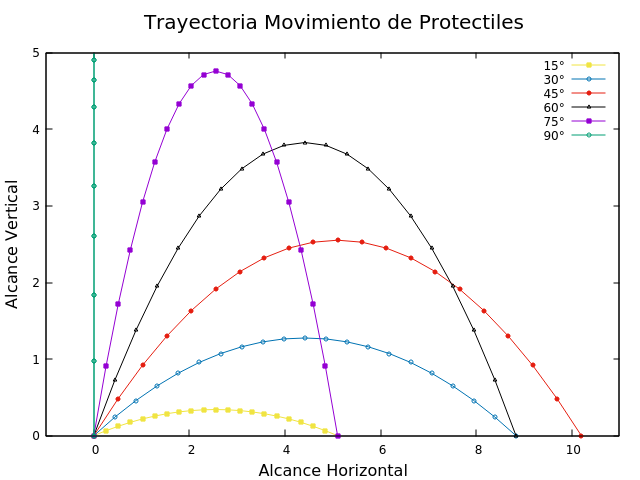
\includegraphics[width=8cm]{Trayectoriaproyectiles.png} 
\caption{Trayectoria de un proyectil en función del ángulo ($\theta$)}\label{fig:figura1}
\end{figure}
\section{Aplicacíon Fortran}
La aplicación Fortran empleado para obtener el conjunto de datos para los ángulos especificados, corresponde a:
\begin{verbatim}
program projectile
  implicit none

  ! definimos constantes
  real, parameter :: g = 9.8
  real, parameter :: pi = 3.1415927
  
  ! definimos las variables
  real :: a, tv, v 
  real, dimension(20):: t=0.,x=0., y=0.
  integer::i,j,nps

  ! Leer valores para el ángulo a, y la velocidad inicial u desde la terminal
  
  write(*,*) 'MOVIMIENTO PARABÓLICO'
  write(*,*) 'DATOS DESPLAZAMIENTO VERTICAL Y HORIZONTAL'
  write(*,*) 'Introduzca los valores de  la velocidad inicial (v) en m&
       &/s y el número de datos'
  read(*,*) v,nps

  !Definimoos el Loop
  loopangulo:do j=15,90,15
     ! convirtiendo ángulo a radianes
     a = j * pi / 180.0
     ! las ecuación para el cálculo del tiempo de vuelo

     tv=2*v*sin(a)/g
  loopposicion: do i=0,nps
     t(i)=t(i)+i*(tv/real(nps))
     x(i)=x(i)+v*t(i)*cos(a)
     y(i)=y(i)+(2*v*t(i)*sin(a)-g*t(i)**2)/2
     ! output data to a file
     open(1, file='datostrayectoria.dat', status='unknown')
     write(1,1000) x(i), y(i)
     1000 format(f15.10,5x,f15.10)
  end do loopposicion
  write(1,1100)
  1100 format(/)
 
  do i=0,nps
     t(i)=0
     x(i)=0
     y(i)=0
     end do
  end do loopangulo
   close(1)

end program projectile

\end{verbatim}
\section{Script Gnuplot}
El script utilizado en la herramienta Gnuplot para graficar los datos obtenidos con la aplicación fortran corresponde al siguiente:
\begin{verbatim}
set title "Trayectoria Movimiento de Protectiles"
set title font ",15" norotate
set xlabel "Alcance Horizontal"
set xlabel font "Verdana,12"
set ylabel "Alcance Vertical"
set ylabel font "Verdana,12"
set style data points
set xrange [-1:11]
set yrange [0:5]
set pointsize 0.7
plot "datostrayectoria.dat" index 0 using 1:2  with linespoints ls 5 title "15°",\
"datostrayectoria.dat" index 1 using 1:2  with linespoints ls 6 title "30°",\
"datostrayectoria.dat" index 2 using 1:2  with linespoints ls 7 title "45°",\
"datostrayectoria.dat" index 3 using 1:2  with linespoints ls 8 title "60°",\
"datostrayectoria.dat" index 4 using 1:2  with linespoints ls 9 title "75°",\
"datostrayectoria.dat" index 5 using 1:2  with linespoints ls 10 title "90°"
\end{verbatim}
\end{document}